\chapter{De Tuckerdecompositie}
\label{hoofdstuk:tucker}

In dit hoofdstuk zullen we verder bouwen op het standaard ST-HOSVD-algoritme om tot een volledig Tucker-gebaseerd compressie-algoritme te komen. Hierbij zullen we de ST-HOSVD versnellen zonder dat de compressie hieronder lijdt, methoden bekijken om orthogonale matrices verder te comprimeren, technieken vergelijken voor het quantizeren van de kerntensor en factormatrices en ten slotte alles lossless comprimeren met Deflate.

\section{Versnellen van de ST-HOSVD}

Hoewel de focus van deze tekst ligt op de afweging tussen de compressiefactor en compressiefout, is het ook nuttig om te kijken naar de compressietijd. In deze sectie zullen enkele technieken besproken worden om de ST-HOSVD te versnellen zonder de fout merkbaar te verhogen.

\subsection{Modevolgorde}

Zoals eerder besproken is het bij de ST-HOSVD van groot belang voor de performantie om de verschillende modes in de juiste volgorde te verwerken. Aangezien we werken met hyperspectrale afbeeldingen, zal de spectrale mode typisch veel beter comprimeren dan de spatiale modes. Ter illustratie: bij het uitvoeren van het standaard ST-HOSVD-algoritme met relatieve doelfout 0.025, comprimeert Cuprite van rang $512 \times 614 \times 190$ naar de volgende rang:
\begin{table}[H]
\centering
\begin{tabular}{|l|l|}
\hline
Modevolgorde & Compressierang \\ \hline
\input{data/modevolgorde.tex}
\end{tabular}
\end{table}
De spectrale dimensie is dus zeker de best comprimeerbare en zal bijgevolg vanaf nu eerst verwerkt worden, gevolgd door de spatiale dimensies (gerangschikt van groot naar klein).

\subsection{Versnellen van de SVD}

\subsubsection{Gram-matrix}

Een belangrijke eigenschap van de SVD is diens verband met de eigenwaardenontbinding. Wanneer $A = U \Sigma V^T$, dan vormen $U$ en $\Sigma^2$ namelijk respectievelijk de eigenvectoren en eigenwaarden van $A A^T$, ook wel bekend als de Gram-matrix van de rijen van $A$ \cite{ref:svd}. Als $A \in \mathbb{R}^{m \times n}$ met $m \ll n$, dan is $A A^T \in \mathbb{R}^{m \times m}$, wat leidt tot een veel snellere eigenwaardenontbinding dan wanneer men de SVD toepast op de volledige matrix. Bij deze methode moet men wel eerst een matrixvermenigvuldiging uitvoeren met complexiteit $O(m^2 n)$, wat van dezelfde orde is als het normaal berekenen van de SVD \cite{ref:svd}, maar dit kan in de praktijk nog steeds erg nuttig zijn aangezien de matrixvermenigvuldiging een relatief eenvoudige operatie is die al sterk geoptimaliseerd is in libraries als LAPACK \cite{ref:lapack}. Verder kan deze aanpak numerieke problemen opleveren omdat we eerst de invoerdata met zichzelf vermenigvuldigen en op het einde de vierkantswortels trekken van de eigenwaarden, wat de precisie verlaagt, maar in deze toepassing hoeft dit geen probleem te zijn aangezien we de SVD sterk afknotten en dit de grootste fout zal veroorzaken. Voor ons zijn fouten van deze grootte dus irrelevant.\\

Een klein nadeel van deze techniek is dat we de matrix $V$ niet meteen hebben zoals bij het berekenen van een SVD. De matricizatie van de gecomprimeerde data $X_k$ (met compressierang $k$) moet nu dus bepaald worden als $X_k := U_k^T X$ (complexiteit $O(kmn)$) in plaats van $X_k := \Sigma_k V_k$ (complexiteit $O(kn)$), wat een hogere complexiteit heeft, maar dit is slechts een matrixvermenigvuldiging dus dit kost niet zo veel tijd meer.\\

\begin{table}[H]
\centering
\begin{tabular}{|l|l|l|}
\hline
Methode & Relatieve fout & Compressietijd (s)\\ \hline
\input{data/gram-matrix.tex}
\end{tabular}
\caption{Vergelijking tussen de standaard ST-HOSVD en de methode met de Gram-matrix voor Cuprite met relatieve doelfout 0.025 (uitgemiddeld over 10 experimenten).}
\end{table}
Dit voorbeeld bevestigt dus dat deze methode een grote versnelling kan opleveren zonder enige significante fout te introduceren.

\subsubsection{Gram-matrix met QR-decompositie}

Om de eventuele fout die veroorzaakt wordt door te werken met de Gram-matrix te verkleinen, is het een gekende techniek om eerst een QR-decompositie van $A^T$ berekenen. Hoewel we eerder bespraken dat deze fout voor onze toepassing minimaal is, is deze techniek in het algemeen interessant om naar te kijken indien het niet veel extra rekentijd kost. In dit geval berekent men eerst $A^T = QR$ en gebruikt men dan de matrix $A A^T = R^T Q^T Q R = R^T R$ in plaats van $A A^T$ als invoer voor de eigenwaardenontbinding.\\

\begin{table}[H]
\centering
\begin{tabular}{|l|l|l|}
\hline
Methode & Relatieve fout & Compressietijd (s)\\ \hline
\input{data/gram-matrix-qr.tex}
\end{tabular}
\caption{Vergelijking tussen de methode met de Gram-matrix met en zonder QR-decompositie voor Cuprite met relatieve doelfout 0.025 (uitgemiddeld over 10 experimenten).}
\end{table}

Men ziet dat de QR-decompositie veel rekentijd kost en zoals eerder vermeld is de fout ge\"introduceerd door de methode met de Gram-matrix toch al verwaarloosbaar. Er is dus geen significant verschil in de relatieve fout. Bijgevolg is deze techniek afgeraden voor onze doeleinden.

\subsubsection{Gram-matrix met Lanczos-algoritme}

Het Lanczos-algoritme \cite{ref:lanczos} is een iteratief algoritme om de grootste $k$ eigenwaarden en corresponderende eigenvectoren te vinden van een symmetrische matrix. Chen en Saad \cite{ref:saad} hebben getoond dat dit algoritme aangepast kan worden om specifiek te werken met Gram-matrices:\\

\begin{algorithm}[H]
\KwData{$A, k, q_1$}
\KwResult{$q_i$'s, $\alpha_i$'s, $\beta_i$'s}
$\beta_1 := 0$\\
$q_0 := 0$\\
\For{$i = 1, ..., k$}{
$w_i := A (A^T q_i) - \beta_i q_{i-1}$\\
$\alpha_i := \langle w_i, q_i \rangle$\\
$w_i := w_i - \alpha_i q_i$\\
$w_i := w_i - \Sigma^{i-1}_{j = 1} \langle w_i q_j \rangle q_j$\\
$\beta_{i+1} := ||w_i||$\\
$q_{i+1} := w_i/\beta_{i+1}$\\
}
\end{algorithm}

De uitvoer hiervan wordt dan samengevoegd in de volgende matrices:

\[
Q = 
\begin{bmatrix}
    q_1 & q_2 & \dots & q_k
\end{bmatrix}
\]
\[
T = \begin{bmatrix}
\alpha_1 & \beta_2 & 0 & \dots & 0 \\
\beta_2 & \alpha_2 & \beta_3 & \dots & 0 \\
0 & \beta_3 & \alpha_3 & \dots & 0 \\
\vdots & \vdots & \vdots & \ddots & \vdots \\
0 & 0 & 0 & \dots & \alpha_k
\end{bmatrix}
\]

Voor elke eigenwaarde en eigenvector $\lambda, x$ van $T$ definieert men de corresponderende Ritz-waarden en Ritz-vectoren als $\lambda, Qx$. Nu geldt dat wanneer men het aantal iteraties $k$ verhoogt, de Ritz-waarden en Ritz-vectoren convergeren naar de grootste $k$ eigenwaarden en bijbehorende eigenvectoren van $A A^T$.\\

Het interessante aan deze methode is dat men slechts $O(mn)$ rekenwerk nodig heeft per iteratie (vanwege de matrix-vectorvermenigvuldiging), dus $O(kmn)$ in totaal, in plaats van de typische $O(min(m, n)mn)$ omdat men geen matrix-matrixvermenigvuldiging meer moet berekenen. Als $k < min(m, n)$ kan men hiermee dus de complexiteit verlagen.\\

Om dit te gebruiken voor onze toepassing, moeten we ons eigen stopcriterion in het algoritme verwerken, door elke iteratie na te kijken of de som van de kwadraten van de $i$ grootste singuliere waarden van $A$ (m.a.w. de som van de $i$ grootste eigenwaarden van $A A^T$) groot genoeg is. Als we dit benaderen met de som van de Ritz-waarden, kan men deze som heel simpel berekenen als $\alpha_1 + \dots + \alpha_i$ (want de som van de eigenwaarden van een matrix is het spoor van de matrix), wat gaat in constante tijd per iteratie. Op deze manier kan men effici\"ent op basis van een doelfout tijdens het algoritme de compressierang kiezen.\\

Ten slotte, eens dat de iteraties be\"eindigd zijn en we een $Q$ en $T$ hebben, berekenen we een eigenwaardenontbinding van $T$ en transformeren de eigenvectoren met $Q$. Voor het berekenen van de eigenwaardenontbinding van een symmetrische tridiagonale $k \times k$ matrix bestaan methoden met complexiteit $O(k^2)$ en er is zelfs onderzoek gedaan naar een algoritme met complexiteit $O(k \log{k})$ \cite{ref:coakley}. Onze implementatie gebruikt de gespecialiseerde functie \texttt{scipy.linalg.eigh\_tridiagonal}, waarvan we vermoeden dat de complexiteit $O(k^2)$ is, maar helaas wordt dit nergens vermeld in de documentatie \cite{ref:eigh_tridiagonal}.

\begin{table}[H]
\centering
\footnotesize
\begin{tabular}{|l|l|l|l|l|}
\hline
Methode & Relatieve fout & Compressietijd (s) & Compressierang & Compressiefactor\\ \hline
\input{data/gram-matrix-lanczos.tex}
\end{tabular}
\normalsize
\caption{Vergelijking tussen de methode met de Gram-matrix met en zonder Lanczos-algoritme voor Cuprite met relatieve doelfout 0.025 (uitgemiddeld over 10 experimenten).}
\end{table}

Blijkbaar convergeert de som van de Ritz-waarden snel genoeg zodat ons stopcriterion de doelfout goed benadert, maar de kwaliteit van de laatste basisvectoren is slechter, waardoor de compressierang significant groter gekozen moet worden voor dezelfde fout en de compressiefactor bijna gehalveerd wordt. Dit wordt ge\"illustreerd in figuur \ref{fig:lanczos-rank-comparison}. De Lanczos-methode geeft dus wel een redelijke basis maar is niet precies genoeg voor onze toepassing. Men zou kunnen proberen dit te verhelpen door meer iteraties uit te voeren dan de compressierang, maar de rekentijd ligt met het huidige aantal iteraties al significant hoger door de extra overhead. Om deze redenen zullen we deze methode verder niet gebruiken.

\begin{figure}[H]
  \centering
  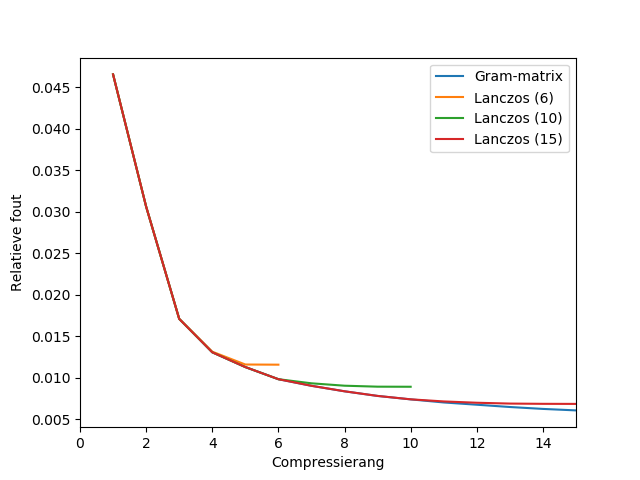
\includegraphics[scale=0.8]{images/lanczos_rank_comparison.png}
  \caption{Relatieve fout voor verschillende compressierangen en methoden bij het comprimeren van de eerste mode (de spectrale mode) van Cuprite. De getallen in de legende geven aan hoeveel Lanczos-iteraties uitgevoerd werden. Men ziet dat het nuttig kan zijn om meer iteraties uit te voeren dan de uiteindelijke compressierang.}
\label{fig:lanczos-rank-comparison}
\end{figure}

\subsubsection{Randomized SVD}

Wanneer we een afgeknotte SVD zoeken van een matrix $A \in \mathbb{R}^{m \times n}$ met $m \ll n$, zijn we eigenlijk ge\"interesseerd in de belangrijkste linker-singuliere vectoren, of met andere woorden, de beste basisvectoren om de verzameling kolomvectoren van $A$ in voor te stellen. Het is echter logisch dat vaak slechts een kleine deelverzameling van de kolomvectoren van $A$ al representatief is voor de volledige populatie en tot een even goede basis leidt. Op deze manier kan men de rekentijd van de SVD verkleinen zonder een grote fout te introduceren. Deze techniek wordt de \textit{randomized SVD} \cite{ref:randomized_svd} genoemd en wordt voor veel toepassingen gebruikt om de SVD te versnellen.\\

Concreet construeren we bij deze methode dus een matrix met een willekeurige verzameling kolommen van $A$ en berekenen we van deze steekproefmatrix de SVD om zo (de eerste kolommen van) $U$ te benaderen. De $\Sigma$ die hierbij berekend wordt is weliswaar niet accuraat, aangezien deze slechts het aandeel van de singuliere vectoren in de steekproef voorstelt, maar dit kan makkelijk gecorrigeerd worden door deze te vermenigvuldigen met $\sqrt{\frac{\text{populatiegrootte}}{\text{steekproefgrootte}}}$. Hierdoor wordt $\Sigma$ ook goed benaderd en kan deze gebruikt worden om bijvoorbeeld de compressierang te bepalen.\\

Verder kan de de SVD van de steekproefmatrix ook berekend worden met de bovenstaande methoden, om zo een grotere versnelling te bekomen.\\

\begin{table}[]
\centering
\begin{tabular}{|l|l|l|}
\hline
Methode & Gram-matrix & Steekproef + Gram-matrix\\ \hhline{|=|=|=|}
\input{data/randomized-svd-cuprite-test.tex}
\end{tabular}
\caption{Vergelijking tussen een typische uitvoering van de methode met de Gram-matrix met en zonder steekproef voor Cuprite met relatieve doelfout 0.025.}
\label{table:randomized-svd-cuprite-test}
\end{table}

In tabel \ref{table:randomized-svd-cuprite-test} vindt men een typische uitvoering met en zonder steekproef. Als steekproefgrootte per mode nemen we simpelweg 5 keer de originele rang. Merk op dat dit over slechts \'e\'en experiment gaat en men dus best geen conclusies trekt over bijvoorbeeld de absolute uitvoeringstijd. Wel kan men zien dat onze benaderingsmethode voor $\Sigma$ adequate precisie geeft. Verder geeft het gebruik van een steekproef in mode 2 een significante versnelling, terwijl in de andere modes de populatie te klein was ten opzichte van de originele rang om een steekproef te nemen. Uiteindelijk is er geen significante fout ge\"introduceerd door het gebruik van de steekproef.\\

\begin{table}[]
\centering
\begin{tabular}{|l|l|l|}
\hline
Methode & Gram-matrix & Steekproef + Gram-matrix\\ \hline
\input{data/randomized-svd-cuprite-average.tex}
\end{tabular}
\caption{Vergelijking tussen de methode met de Gram-matrix met en zonder steekproef voor Cuprite met relatieve doelfout 0.025 (10 experimenten).}
\label{table:randomized-svd-cuprite-average}
\end{table}

\begin{table}[]
\centering
\begin{tabular}{|l|l|l|}
\hline
Methode & Gram-matrix & Steekproef + Gram-matrix\\ \hline
\input{data/randomized-svd-mauna-kea-average.tex}
\end{tabular}
\caption{Vergelijking tussen de methode met de Gram-matrix met en zonder steekproef voor Mauna Kea met relatieve doelfout 0.025 (10 experimenten).}
\label{table:randomized-svd-mauna-kea-average}
\end{table}

We zien in tabel \ref{table:randomized-svd-cuprite-average} dat, voor deze dataset, de randomized SVD een degelijke versnelling geeft zonder een significant verschil in de fout of compressiefactor. Daarnaast is de variantie op de fout en compressiefactor erg klein. Bovendien toont tabel \ref{table:randomized-svd-mauna-kea-average} aan dat deze techniek ook goed werkt voor voor Mauna Kea, al is het met een steekproef van 20 keer de originele rang.\\

Verder hebben we als kleine optimizatie getest of het sorteren van de steekproefindices voor het selecteren van deze kolommen uit de steekproefmatrix effect heeft op de uitvoeringstijd. Dit kost rekenwerk maar kan eventueel een versnelling geven bij het kopi\"eren van de kolommen vanwege het betere \textit{memory access pattern}. In de praktijk bleef de rekentijd ongeveer hetzelfde, dus we gebruiken deze techniek verder niet.\\

\begin{figure}[]
  \centering
  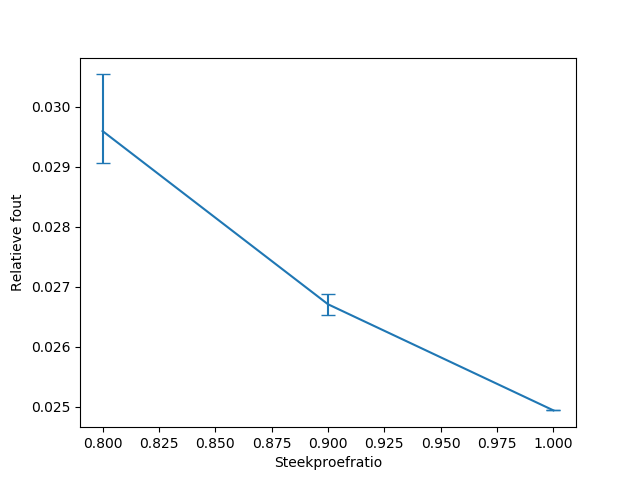
\includegraphics[scale=0.8]{images/randomized_svd_pavia_ratios.png}
  \caption{Compressiefout bij verschillende steekproefratios voor Pavia Centra met relatieve doelfout 0.025 (uitgemiddeld over 3 experimenten). De foutbalkjes stellen de minimale en maximale waarden voor over de verschillende experimenten.}
\label{fig:randomized-svd-pavia-ratios}
\end{figure}

In figuur \ref{fig:randomized-svd-pavia-ratios} ziet men echter dat de randomized SVD geen goede resultaten geeft bij Pavia Centre. Hierbij moesten we de steekproefratio (de verhouding tussen de steekproefgrootte en populatiegrootte) verhogen tot 1 om geen merkbare fout toe te voegen, maar in tabel \ref{table:randomized-svd-pavia-test} zien we dat een steekproefratio van 0.2 nog redelijk lijkt te werken voor de spectrale mode, de best comprimeerbare mode. Daarnaast zijn alle modes van Pavia significant slechter comprimeerbaar dan die van Cuprite. Hierdoor denken we dat de steekproefgrootte best groter gekozen wordt wanneer de mode slecht comprimeerbaar is.\\

De meest logische manier om de ``comprimeerbaarheid'' van een mode in te schatten, is echter door te kijken naar de verdeling van de singuliere waarden, die men pas kent na het berekenen van de SVD. Het lijkt ons dus moeilijk om voor een brede verzameling datasets op consistente wijze snel een goede steekproefgrootte te kiezen zonder verdere gegevens over de data, hoewel dit mogelijk verder onderzocht kan worden. Om deze reden zullen we de randomized SVD verder niet gebruiken, hoewel ze voor bepaalde datasets zeker een mooie versnelling kan opleveren.

\subsubsection{Besluit}

Na de resultaten van alle bovenstaande methodes te vergelijken, kiezen we ervoor om vanaf nu de methode met de Gram-matrix zonder verdere toevoegingen te gebruiken voor het berekenen van de SVD. Dit lijkt ons de snelste methode die geen significant effect heeft op de compressiefout- of factor.

\begin{table}[H]
\centering
\begin{tabular}{|l|l|l|}
\hline
Methode & Gram-matrix & Steekproef + Gram-matrix\\ \hhline{|=|=|=|}
\input{data/randomized-svd-pavia-test.tex}
\end{tabular}
\caption{Vergelijking tussen een uitvoering van de methode met de Gram-matrix met en zonder steekproef voor Pavia Centre met relatieve doelfout 0.025.}
\label{table:randomized-svd-pavia-test}
\end{table}
\section{Orthogonaliteitscompressie}

Men zou kunnen denken dat bij de Tuckerdecompositie de meeste ruimte ingenomen wordt door de kerntensor. Wanneer men namelijk naar tensoren met $k$ modes kijkt, waarbij de lengte per mode $n$ constant blijft en telkens gecomprimeerd wordt naar constante rang $r$, dan groeit de gecomprimeerde kerntensor met $O(r^k)$ en de factormatrices slechts met $O(knr)$, dus met $n, r$ constant en groeiende $k$ worden de factormatrices verwaarloosbaar.\\

In de praktijk werken we echter met een beperkt aantal modes en vaak lage compressierangen. Zelfs als we later reshapen verhogen we hiermeee $k$, maar verlagen we $n$ en $r$, dus het aandeel van de kerntensor zal hierdoor niet zozeer veel verhogen. Bijvoorbeeld, wanneer men de ST-HOSVD toepast op Cuprite met relatieve doelfout 0.025, comprimeert men van rang (512, 614, 190) naar (139, 192, 4) en nemen de factormatrices 64\% van het geheugen in. Bij Mauna Kea, een veel grotere dataset, is dit percentage 55\%. We kunnen dus concluderen dat het zeker interessant is om te kijken naar specifieke compressietechnieken voor de factormatrices.\\

We weten dat de factormatrices orthogonaal zijn en dit kunnen we benutten. Stel namelijk, we hebben een factormatrix $U \in \mathbb{R}^{n \times r}$ en verdelen deze op de volgende wijze:
\[
U = \begin{bmatrix}
A & c & \dots \\
B & x & \dots \\
\end{bmatrix}
\]
met $A \in \mathbb{R}^{(n-k) \times k}$, $B \in \mathbb{R}^{k \times k}$, $c \in \mathbb{R}^{n-k}$, $x \in \mathbb{R}^{k}$, voor willekeurige $1 \leq k < n$. Vanwege orthogonaliteit weten we dat:
\begin{align*}
\begin{bmatrix}
A \\
B \\
\end{bmatrix}^T
\begin{bmatrix}
c \\
x \\
\end{bmatrix}
&= 0 \\
A^T c + B^T x &= 0 \\
B^T x &= -A^T c
\end{align*}
Bijgevolg kunnen we $x$ berekenen als de oplossing van een lineair stelsel met $k$ onafhankelijke vergelijkingen en $k$ variabelen en moeten deze waarden niet opgeslagen worden. Theoretisch gezien kan men dus, door dit proces sequentieel uit te voeren voor $k = 1, \dots, n - 1$, een hele driehoek van $r (r - 1)/2$ elementen uit de matrix laten vallen. Om terug te komen op de eerdere voorbeelden: dit zou bij Cuprite en Mauna Kea neerkomen op 9.4\% en 7.5\% van alle waarden (inclusief kerntensor) respectievelijk. Men kan ook kiezen om de kolommen in een andere volgorde te verwerken, maar dit leek ons het beste zodat de herberekende waarden vooral zitten in de latere singuliere vectoren, die minder belangrijk zijn.

\section{Quantizatie}

\section{Bitstring-compressie}